\ifx\allfiles\undefined
\documentclass[UTF8]{ctexart}
\title{以太坊挖共识算法与挖矿激励}
\author{邹远春}
\date{}
\usepackage{xeCJK}
\usepackage{graphicx}
\usepackage{listings}
\usepackage{verbatim}
\usepackage{graphicx}
\usepackage{xcolor}
\usepackage{listings}
\usepackage{amsmath}
\lstset{%
	breaklines=true,
	tabsize=2
}
\begin{document}
\maketitle
\newcommand\Emph{\textbf}
\else
\chapter{以太坊挖共识算法与挖矿激励}
\fi

本篇介绍了挖掘一个新区块在代码上的完整过程,从调用函数入口开始,沿调用过程一路向深,直至最终完成新区块授权/封印的共识算法,并对两种共识算法的设计思路和实现细节都进行了详细讲解。


\section{miner相关UML结构}

详情参考:[以太坊源代码分析]III. 挖矿和共识算法的奥秘 

https://blog.csdn.net/teaspring/article/details/78050274

\section{待挖掘区块需要组装}

在Ethereum 代码中,名为miner的包(package)负责向外提供一个“挖矿”得到的新区块,其主要结构体的UML关系图如下图所示:

\begin{figure}
	\centering
	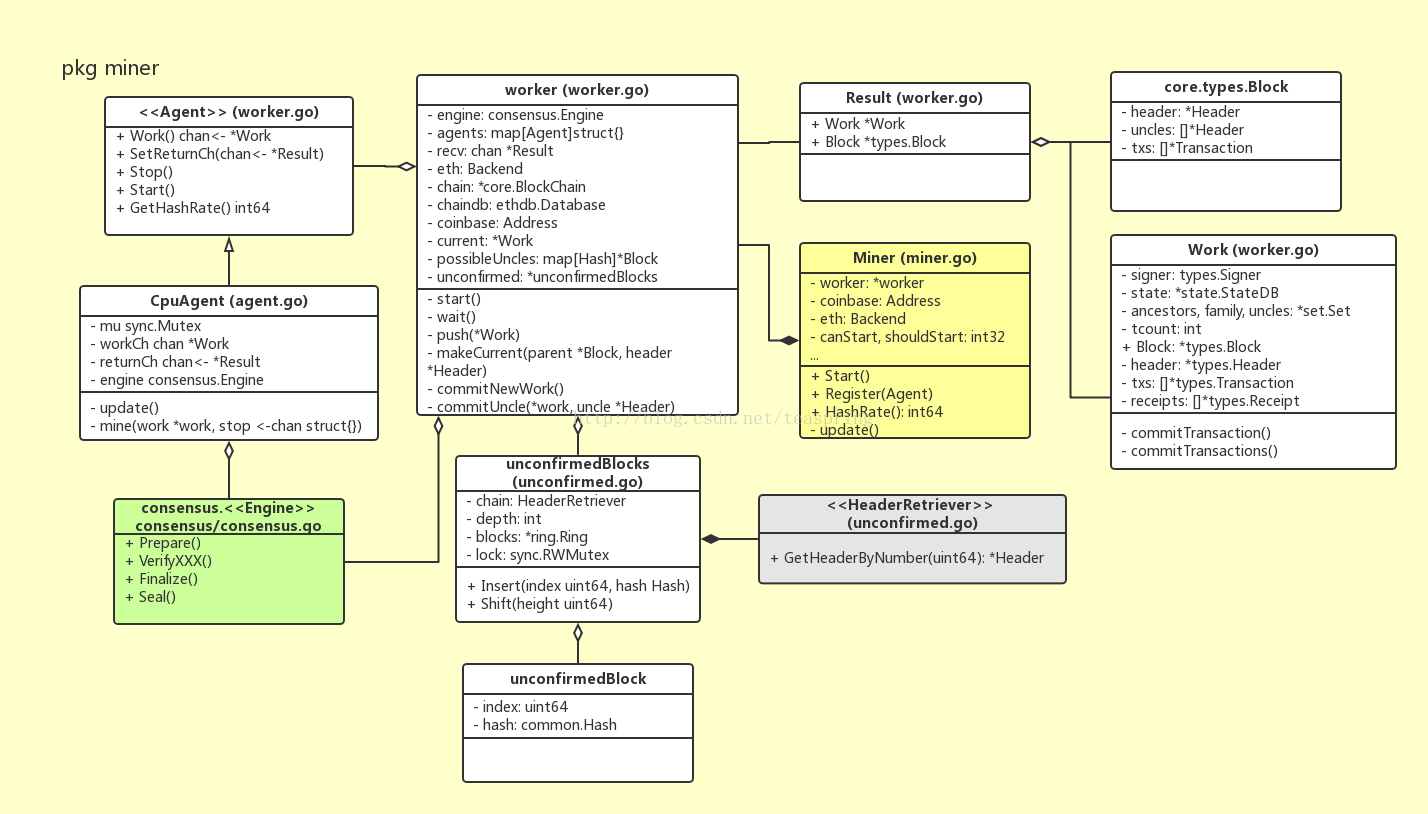
\includegraphics[scale=0.3]{miner.png}
	\caption{Miner}
	\label{miner}
\end{figure}

处于入口的类是Miner,它作为公共类型,向外暴露mine功能;它有一个worker类型的成员变量,负责管理mine过程;worker内部有一组Agent接口类型对象,每个Agent都可以完成单个区块的mine,目测这些Agent之间应该是竞争关系;Work结构体主要用以携带数据,被视为挖掘一个区块时所需的数据环境。

主要的数据传输发生在worker和它的Agent(们)之间:在合适的时候,worker把一个Work对象发送给每个Agent,然后任何一个Agent完成mine时,将一个经过授权确认的Block加上那个更新过的Work,组成一个Result对象发送回worker。

有意思的是<<Agent>>接口,尽管调用方worker内部声明了一个Agent数组,但目前只有一个实现类CpuAgent的对象会被加到该数组,可能这个Agent数组是为将来的扩展作的预留吧。CpuAgent通过全局的<<Engine>>对象,借助共识算法完成最终的区块授权。

另外,unconfirmedBlocks 也挺特别,它会以unconfirmedBlock的形式存储最近一些本地挖掘出的区块。在一段时间之后,根据区块的Number和Hash,再确定这些区块是否已经被收纳进主干链(canonical chain)里,以输出Log的方式来告知用户。

对于一个新区块被挖掘出的过程,代码实现上基本分为两个环节:一是组装出一个新区块,这个区块的数据基本完整,包括成员Header的部分属性,以及交易列表txs,和叔区块组uncles[],并且所有交易已经执行完毕,所有收据(Receipt)也已收集完毕,这部分主要由worker完成;二是填补该区块剩余的成员属性,比如Header.Difficulty等,并完成授权,这些工作是由Agent调用<Engine>接口实现体,利用共识算法来完成的。

\paragraph{新区块的组装流程}

挖掘新区块的流程入口在Miner里,略显奇葩的是,具体入口在Miner结构体的创建函数(避免称之为‘构造函数’)里。

\begin{figure}
	\centering
	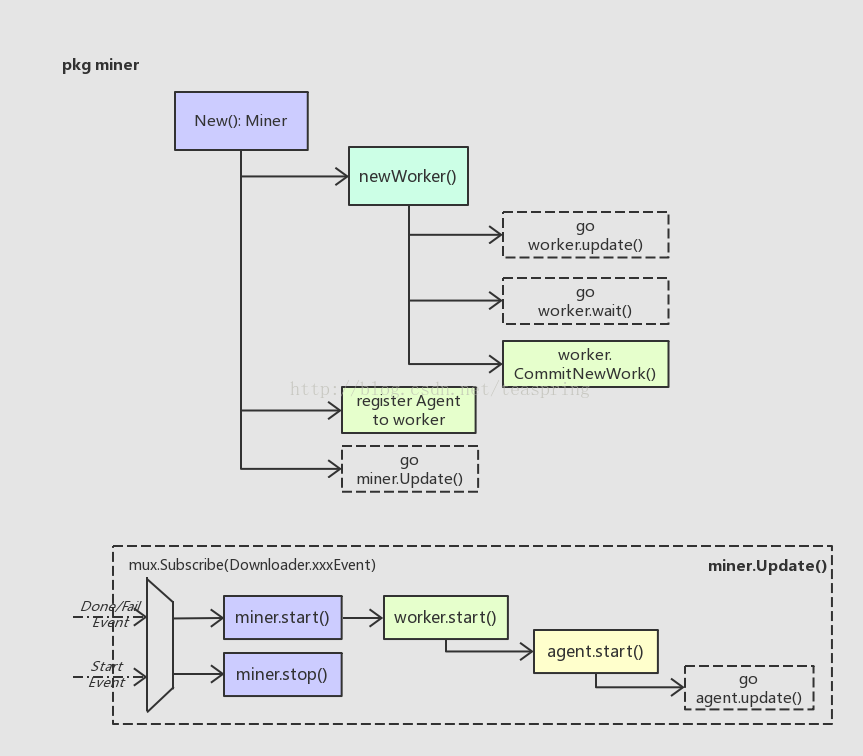
\includegraphics[scale=0.5]{newMiner.png}
	\caption{New Miner}
	\label{newMiner}
\end{figure}

\paragraph{Miner的函数}

\subparagraph{New()}

在New()里,针对新对象miner的各个成员变量初始化完成后,会紧跟着创建worker对象,然后将Agent对象登记给worker,最后用一个单独线程去运行miner.Update()函数;而worker的创建函数里也如法炮制,分别用单独线程去启动worker.updater()和wait();最后worker.CommitNewWork()会开始准备一个新区块所需的基本数据,如Header,Txs, Uncles等。注意此时Agent尚未启动。

\subparagraph{Update()}

这个update()会订阅(监听)几种事件,均跟Downloader相关。当收到Downloader的StartEvent时,意味者此时本节点正在从其他节点下载新区块,这时miner会立即停止进行中的挖掘工作,并继续监听;如果收到DoneEvent或FailEvent时,意味本节点的下载任务已结束-无论下载成功或失败-此时都可以开始挖掘新区块,并且此时会退出Downloader事件的监听。

从miner.Update()的逻辑可以看出,对于任何一个Ethereum网络中的节点来说,挖掘一个新区块和从其他节点下载、同步一个新区块,根本是相互冲突的。这样的规定,保证了在某个节点上,一个新区块只可能有一种来源,这可以大大降低可能出现的区块冲突,并避免全网中计算资源的浪费。

\subparagraph{worker的函数}
这里我们主要关注worker.updater()和wait()

\begin{figure}
	\centering
	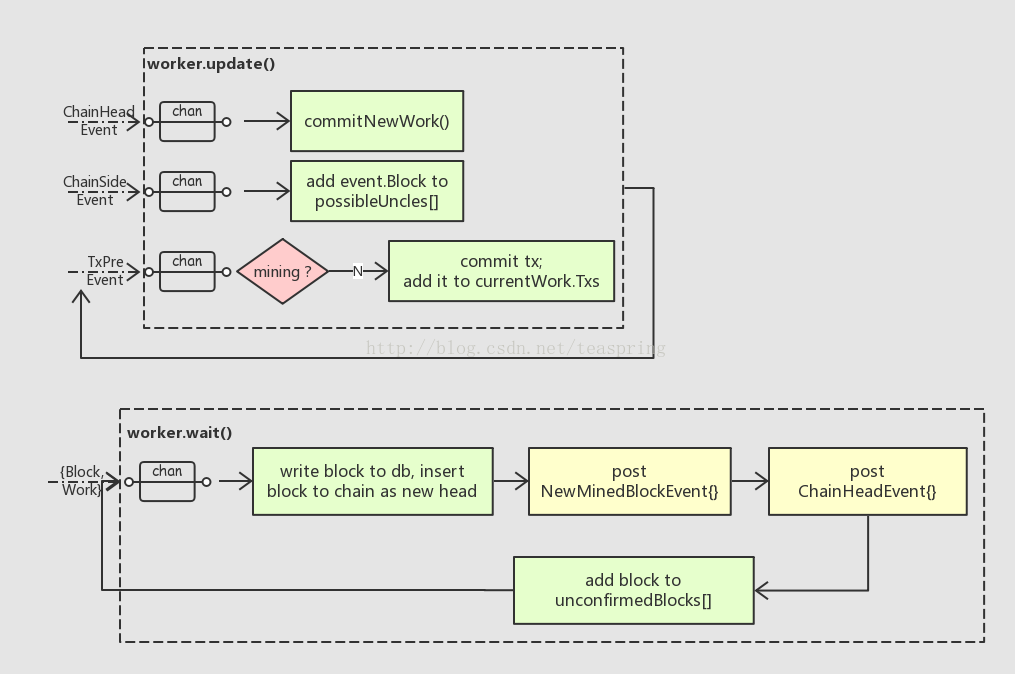
\includegraphics[scale=0.4]{worker.png}
	\caption{worker}
	\label{worker}
\end{figure}

\subparagraph{update()}

worker.update()分别监听ChainHeadEvent,ChainSideEvent,TxPreEvent几个事件,每个事件会触发worker不同的反应。ChainHeadEvent是指区块链中已经加入了一个新的区块作为整个链的链头,这时worker的回应是立即开始准备挖掘下一个新区块(也是够忙的);ChainSideEvent指区块链中加入了一个新区块作为当前链头的旁支,worker会把这个区块收纳进possibleUncles[]数组,作为下一个挖掘新区块可能的Uncle之一;TxPreEvent是TxPool对象发出的,指的是一个新的交易tx被加入了TxPool,这时如果worker没有处于挖掘中,那么就去执行这个tx,并把它收纳进Work.txs数组,为下次挖掘新区块备用。

需要稍稍注意的是,ChainHeadEvent并不一定是外部源发出。由于worker对象有个成员变量chain(eth.BlockChain),所以当worker自己完成挖掘一个新区块,并把它写入数据库,加进区块链里成为新的链头时,worker自己也可以调用chain发出一个ChainHeadEvent,从而被worker.update()函数监听到,进入下一次区块挖掘。

\subparagraph{wait()}

worker.wait()会在一个channel处一直等待Agent完成挖掘发送回来的新Block和Work对象。这个Block会被写入数据库,加入本地的区块链试图成为最新的链头。注意,此时区块中的所有交易,假设都已经被执行过了,所以这里的操作,不会再去执行这些交易对象。

当这一切都完成,worker就会发送一条事件(NewMinedBlockEvent{}),等于通告天下:我挖出了一个新区块!这样监听到该事件的其他节点,就会根据自身的状况,来决定是否接受这个新区块成为全网中公认的区块链新的链头。至于这个公认过程如何实现,就属于共识算法的范畴了。

\subparagraph{commitNewWork()}

commitNewWork()会在worker内部多处被调用,注意它每次都是被直接调用,并没有以goroutine的方式启动。commitNewWork()内部使用sync.Mutex对全部操作做了隔离。这个函数的基本逻辑如下:

\begin{itemize}

\item 准备新区块的时间属性Header.Time,一般均等于系统当前时间,不过要确保父区块的时间(parentBlock.Time())要早于新区块的时间,父区块当然来自当前区块链的链头了。

\item 创建新区块的Header对象,其各属性中:Num可确定(父区块Num +1);Time可确定;ParentHash可确定;其余诸如Difficulty,GasLimit等,均留待之后共识算法中确定。

\item 调用Engine.Prepare()函数,完成Header对象的准备。

\item 根据新区块的位置(Number),查看它是否处于DAO硬分叉的影响范围内,如果是,则赋值予header.Extra。

\item 根据已有的Header对象,创建一个新的Work对象,并用其更新worker.current成员变量。

\item 如果配置信息中支持硬分叉,在Work对象的StateDB里应用硬分叉。

\item 准备新区块的交易列表,来源是TxPool中那些最近加入的tx,并执行这些交易。

\item 准备新区块的叔区块uncles[],来源是worker.possibleUncles[],而possibleUncles[]中的每个区块都从事件ChainSideEvent中搜集得到。注意叔区块最多有两个。

\item 调用Engine.Finalize()函数,对新区块“定型”,填充上Header.Root, TxHash, ReceiptHash, UncleHash等几个属性。

\item 如果上一个区块(即旧的链头区块)处于unconfirmedBlocks中,意味着它也是由本节点挖掘出来的,尝试去验证它已经被吸纳进主干链中。

\item 把创建的Work对象,通过channel发送给每一个登记过的Agent,进行后续的挖掘。

\end{itemize}

以上步骤中,4和6都是仅仅在该区块配置中支持DAO硬分叉,并且该区块的位置正好处于DAO硬分叉影响范围内时才会发生;其他步骤是普遍性的。commitNewWork()完成了待挖掘区块的组装,block.Header创建完毕,交易数组txs,叔区块Uncles[]都已取得,并且由于所有交易被执行完毕,相应的Receipt[]也已获得。万事俱备,可以交给Agent进行‘挖掘’了。

\paragraph{CpuAgent的函数}

CpuAgent中与mine相关的函数,主要是update()和mine():

\begin{figure}
	\centering
	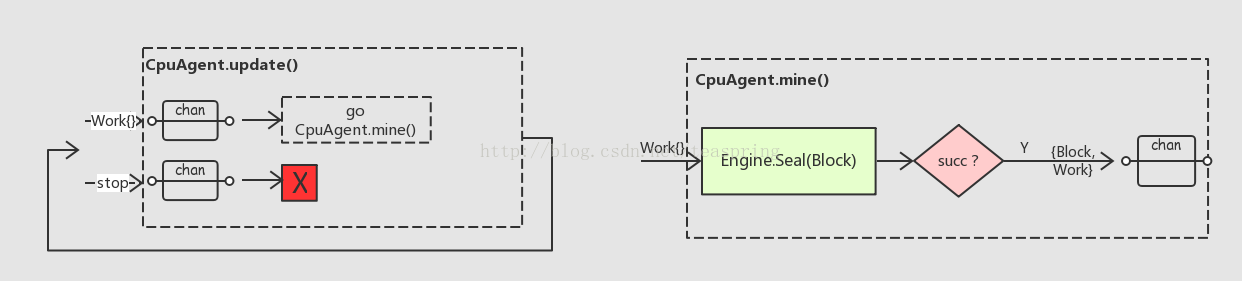
\includegraphics[scale=0.3]{cpuagent.png}
	\caption{Cpu Agent}
	\label{cpuAgent}
\end{figure}

\subparagraph{CpuAgent.update()}就是worker.commitNewWork()结束后发出Work对象的会一直监听相关channel,如果收到Work对象(显然由worker.commitNewWork()结束后发出),就启动mine()函数;如果收到停止(mine)的消息,就退出一切相关操作。

\subparagraph{CpuAgent.mine()}会直接调用Engine.Seal()函数,利用Engine实现体的共识算法对传入的Block进行最终的授权,如果成功,就将Block同Work一起通过channel发还给worker,那边worker.wait()会接收并处理。

显然,这两个函数都没做什么实质性工作,它们只是负责调用<Engine>接口实现体,待授权完成后将区块数据发送回worker。挖掘出一个区块的真正奥妙全在Engine实现体所代表的共识算法里。

\section{共识算法完成挖掘}

共识算法族对外暴露的是Engine接口,其有两种实现体,分别是基于运算能力的Ethash算法和基于“同行”认证的的Clique算法。

\begin{figure}
	\centering
	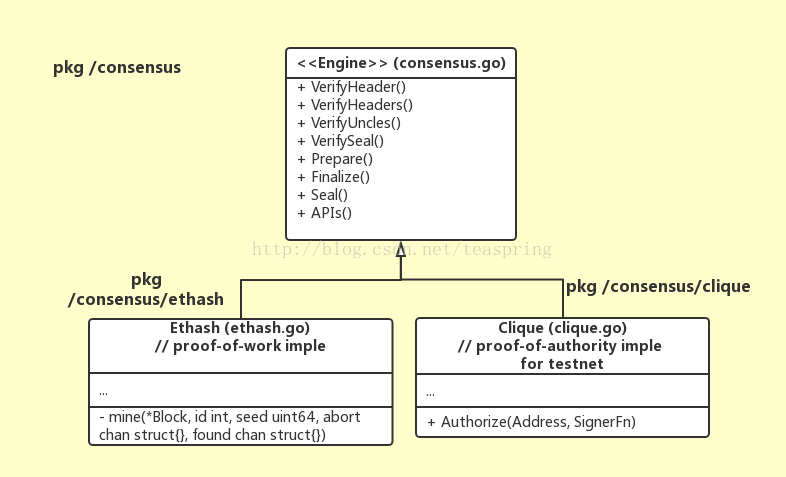
\includegraphics[scale=0.5]{consensus.png}
	\caption{consensus}
	\label{consensus}
\end{figure}

在Engine接口的声明函数中,VerifyHeader(),VerifyHeaders(),VerifyUncles()用来验证区块相应数据成员是否合理合规,可否放入区块;Prepare()函数往往在Header创建时调用,用来对Header.Difficulty等属性赋值;Finalize()函数在区块区块的数据成员都已具备时被调用,比如叔区块(uncles)已经具备,全部交易Transactions已经执行完毕,全部收据(Receipt[])也已收集完毕,此时Finalize()会最终生成Root,TxHash,UncleHash,ReceiptHash等成员。

而Seal()和VerifySeal()是Engine接口所有函数中最重要的。Seal()函数可对一个调用过Finalize()的区块进行授权或封印,并将封印过程产生的一些值赋予区块中剩余尚未赋值的成员(Header.Nonce, Header.MixDigest)。Seal()成功时返回的区块全部成员齐整,可视为一个正常区块,可被广播到整个网络中,也可以被插入区块链等。所以,对于挖掘一个新区块来说,所有相关代码里Engine.Seal()是其中最重要,也是最复杂的一步。VerifySeal()函数基于跟Seal()完全一样的算法原理,通过验证区块的某些属性(Header.Nonce,Header.MixDigest等)是否正确,来确定该区块是否已经经过Seal操作。

在两种共识算法的实现中,Ethash是产品环境下以太坊真正使用的共识算法,Clique主要针对以太坊的测试网络运作,两种共识算法的差异,主要体现在Seal()的实现上。

\paragraph{Ethash共识算法}

Ethash算法又被称为Proof-of-Work(PoW),是基于运算能力的授权/封印过程。Ethash实现的Seal()函数,其基本原理可简单表示成以下公式:

\begin{center}
$RAND(h, n) <= M / d$
\end{center}

这里M表示一个极大的数,比如$2^{256}-1$;d表示Header成员Difficulty。RAND()是一个概念函数,它代表了一系列复杂的运算,并最终产生一个类似随机的数。这个函数包括两个基本入参:h是Header的哈希值(Header.HashNoNonce()),n表示Header成员Nonce。整个关系式可以大致理解为,在最大不超过M的范围内,以某个方式试图找到一个数,如果这个数符合条件(<=M/d),那么就认为Seal()成功。

我们可以先定性的验证一个\Emph{推论:d的大小对整个关系式的影响}。假设h,n均不变,如果d变大,则M/d变小,那么对于RAND()生成一个满足该条件的数值,显然其概率是下降的,即意味着难度将加大。考虑到以上变量的含义,当Header.Difficulty逐渐变大时,这个对应区块被挖掘出的难度(恰为Difficulty本义)也在缓慢增大,挖掘所需时间也在增长,所以上述推论是合理的。

\subparagraph{mine()函数}
Ethash.Seal()函数实现中,会以多线程(goroutine)的方式并行调用mine()函数,线程个数等于Ethash.threads;如果Ethash.threads被设为0,则Ethash选择以本地CPU中的总核数作为开启线程的个数。

\begin{lstlisting}

/* consensus/ethash/sealer.go */
func (ethash *Ethash) mine(block *Block, id int, seed uint64, abort chan struct{}, found chan *Block) {
    var (
        header = block.Header()
        hash   = header.HashNoNonce().Bytes()
        target = new(big.Int).Div(maxUint256, header.Difficulty)
        number = header.Number.Uint64()
        dataset = ethash.dataset(number)
        nonce  = seed
    )
    for {
        select {
        case <-abort:
            ...; return
        default:
            digest, result := hashimotoFull(dataset, hash, nonce) // compute the PoW value of this nonce
            if new(big.Int).SetBytes(result).Cmp(target) <= 0 { // x.Cmp(y) <= 0 means x <= y
                header = types.CopyHeader(header)
                header.Nonce = types.EncodeNonce(nonce)
                header.MixDigest = common.BytesToHash(digest)
                found<- block.WithSeal(header)
                return
            }
        }
        nonce++
    }
}

\end{lstlisting}


以上代码就是mine()函数的主要业务逻辑。入参@id是线程编号,用来发送log告知上层;函数内部首先定义一组局部变量,包括之后调用hashimotoFull()时传入的hash、nonce、巨大的辅助数组dataset,以及结果比较的target;然后是一个无限循环,每次调用hashimotoFull()进行一系列复杂运算,一旦它的返回值符合条件,就复制Header对象(深度拷贝),并赋值Nonce、MixDigest属性,返回经过授权的区块。注意到在每次循环运算时,nonce还会自增+1,使得每次循环中的计算都各不相同。

这里hashimotoFull()函数通过调用hashimoto()函数完成运算,而同时还有另外一个类似的函数hashimoLight()函数。

\begin{lstlisting}

func hashimotoFull(dataset []uint32, hash []byte, nonce uint64) ([]byte, []byte) {
    lookup := func(index uint32) []uint32 {
        offset := index * hashWords
        return dataset[offset : offset+hashWords]
    }
    return hashimoto(hash, nonce, uint64(len(dataset))*4, lookup)
}
func hashimotoLight(size uint64, cache []uint32, hash []byte, nonce uint64) ([]byte, []byte) {
    lookup := func(index uint32) []uint32 {
        rawData := generateDatasetItem(cache, index, keccak512)
        data := make([]uint32, len(rawData)/4)
        for i := 0; i < len(data); i++ {
            data[i] = binary.LittleEndian.Uint32(rawData[i*4:])
        }
        return data
    }
    return hashimoto(hash, nonce, size, lookup)
}

\end{lstlisting}

以上两个函数,最终都调用了hashimoto()。它们的差别,在于各自调用hashimoto()函数的入参@size uint 和 @lookup func()不同。相比于Light(),Full()函数调用的size更大,以及一个从更大数组中获取数据的查询函数lookup()。\Emph{hashimotoFull()函数是被Seal()调用的},而hashimotoLight()是为VerifySeal()准备的。

这里的lookup()函数其实很重要,它其实是一个以非线性表查找方式进行的哈希函数! 这种哈希函数的性能不仅取决于查找的逻辑,更多的依赖于所查找的表格的数据规模大小。lookup()会以函数型参数的形式传递给hashimoto()

\Emph{核心的运算函数hashimoto()}

最终为Ethash共识算法的Seal过程执行运算任务的是hashimoto()函数,它的函数类型如下:

\begin{lstlisting}
// consensus/ethash/algorithm.go
func hashimoto(hash []byte, nonce uint64, size uint64, lookup(index uint32) []uint32) (digest []byte, result []byte)
\end{lstlisting}

hashimoto()函数的入参包括:区块哈希值@hash, 区块nonce成员@nonce,和非线性表查找的哈希函数lookup(),及其所查找的非线性表格的容量@size。返回值digest和result,都是32 bytes长的字节串。
hashimoto()的逻辑比较复杂,包含了多次、多种哈希运算。下面尝试从其中数据结构变化的角度来简单描述之:


\begin{figure}
	\centering
	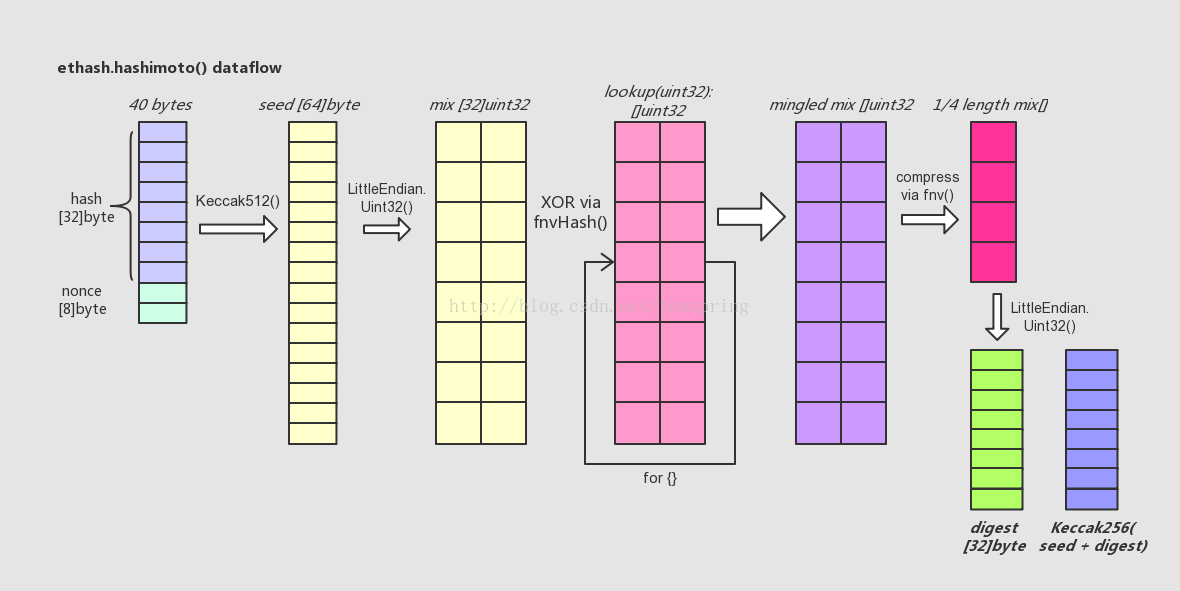
\includegraphics[scale=0.3]{hashimoto.png}
	\caption{hashimoto}
	\label{hashimoto}
\end{figure}


简单介绍一下上图所代表的代码流程:

\begin{itemize}

\item 首先,hashimoto()函数将入参@hash和@nonce合并成一个40 bytes长的数组,取它的SHA-512哈希值取名seed,长度为64 bytes。

\item 然后,将seed[]转化成以uint32为元素的数组mix[],注意一个uint32数等于4 bytes,故而seed[]只能转化成16个uint32数,而mix[]数组长度32,所以此时mix[]数组前后各半是等值的。

\item 接着,lookup()函数登场。用一个循环,不断调用lookup()从外部数据集中取出uint32元素类型数组,向mix[]数组中混入未知的数据。循环的次数可用参数调节,目前设为64次。每次循环中,变化生成参数index,从而使得每次调用lookup()函数取出的数组都各不相同。这里混入数据的方式是一种类似向量“异或”的操作,来自于FNV算法。

\item 待混淆数据完成后,得到一个基本上面目全非的mix[],长度为32的uint32数组。这时,将其折叠(压缩)成一个长度缩小成原长1/4的uint32数组,折叠的操作方法还是来自FNV算法。

\item 最后,将折叠后的mix[]由长度为8的uint32型数组直接转化成一个长度32的byte数组,这就是返回值@digest;同时将之前的seed[]数组与digest合并再取一次SHA-256哈希值,得到的长度32的byte数组,即返回值@result。
\end{itemize}

最终经过一系列多次、多种的哈希运算,hashimoto()返回两个长度均为32的byte数组 - digest[]和result[]。回忆一下ethash.mine()函数中,对于hashimotoFull()的两个返回值,会直接以big.int整型数形式比较result和target;如果符合要求,则将digest取SHA3-256的哈希值(256 bits),并存于Header.MixDigest中,待以后Ethash.VerifySeal()可以加以验证。

\Emph{以非线性表查找方式进行的哈希运算}

上述hashimoto()函数中,函数型入参lookup()其实表示的是一次以非线性表查找方式进行的哈希运算,lookup()以入参为key,从所关联的数据集中按照定义好的一段逻辑取出64 bytes长的数据作为hash value并返回,注意返回值以uint32的形式则相应变成16个uint32长。返回的数据会在hashimoto()函数被其他的哈希运算所使用。

以非线性表的查找方式进行的哈希运算(hashing by nonlinear table lookup),属于众多哈希函数中的一种实现,在Ethash算法的核心环节有大量使用,所使用到的非线性表被定义成两种结构体,分别叫cache{}和dataset{}。二者的差异主要是表格的规模和调用场景:dataset{}中的数据规模更加巨大,从而会被hashimotoFull()调用从而服务于Ethash.Seal();cache{}内含数据规模相对较小,会被hashimotoLight()调用并服务于Ethash.VerifySeal()。

\begin{figure}
	\centering
	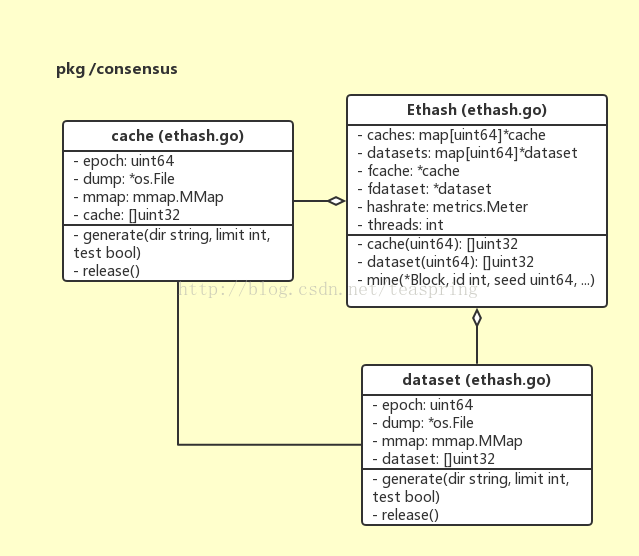
\includegraphics[scale=0.5]{ethash.png}
	\caption{ethash}
	\label{ethash}
\end{figure}


以cache{}的结构体声明为例,成员cache就是实际使用的一块内存Buffer,mmap是内存映射对象,dump是该内存buffer存储于磁盘空间的文件对象,epoch是共享这个cache{}对象的一组区块的序号。从上述UML图来看,cache和dataset的结构体声明基本一样,这也暗示了它们无论是原理还是行为都极为相似。

\Emph{cache\{\}对象的生成}


dataset{}和cache{}的生成过程很类似,都是通过内存映射的方式读/写磁盘文件。

\begin{figure}
	\centering
	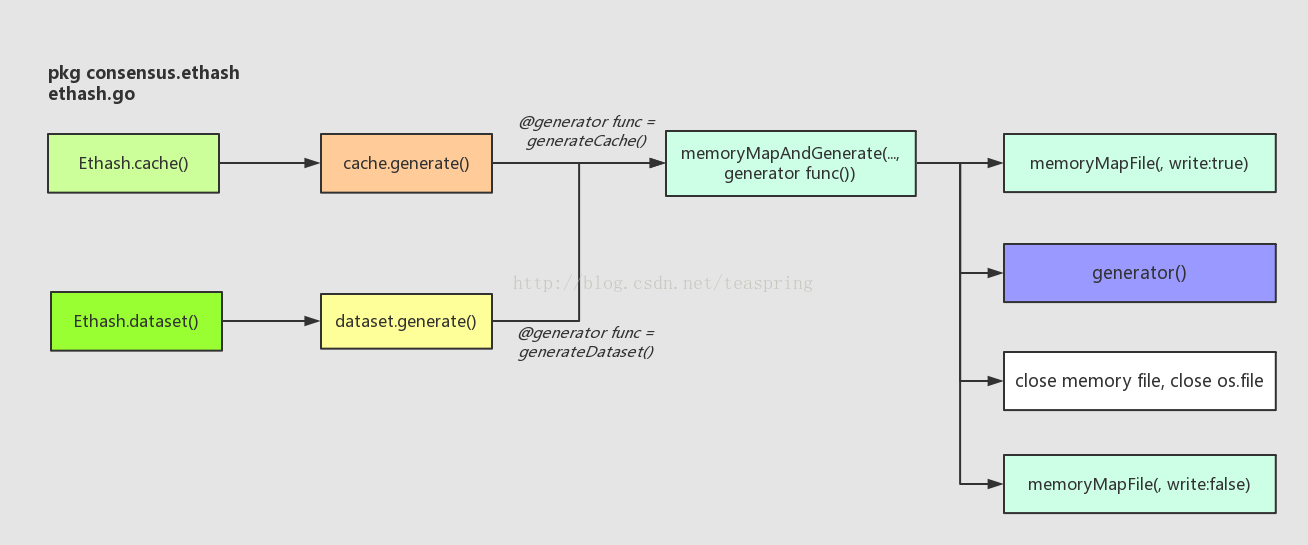
\includegraphics[scale=0.3]{cache.png}
	\caption{cache}
	\label{cache}
\end{figure}

以cache{}为例,Ethash.cache(uint64)会确保该区块所用到的cache{}对象已经创建,它的入参是区块的Number,用Number/epochLength可以得到该区块所对应的epoch号。epochLength被定义成常量30000,意味着每连续30000个区块共享一个cache{}对象。

有意思的是内存映射相关的函数,memoryMapAndGenerate()会首先调用memoryMapFile()生成一个文件并映射到内存中的一个数组,并调用传入的函数型参数generator() 进行数据的填入,于是这个内存数组以及所映射的磁盘文件就同时变得十分巨大,注意此时传入memoryMapFile()的文件操作权限是可写的。然后再关闭所有文件操作符,调用memoryMapFile()重新打开这个磁盘文件并映射到内存的一个数组,注意此时的文件操作权限是只读的。可见这组函数的coding很精细。

Ethash中分别用一个map结构来存放不同epoch对应的cache对象和dataset对象,缓存成员fcache和fdataset,用以提前创建cache{}和dataset{}对象以避免下次使用时再花费时间。

我们以cache{}为例,看看cache.generate()方法的具体逻辑:

\begin{figure}
	\centering
	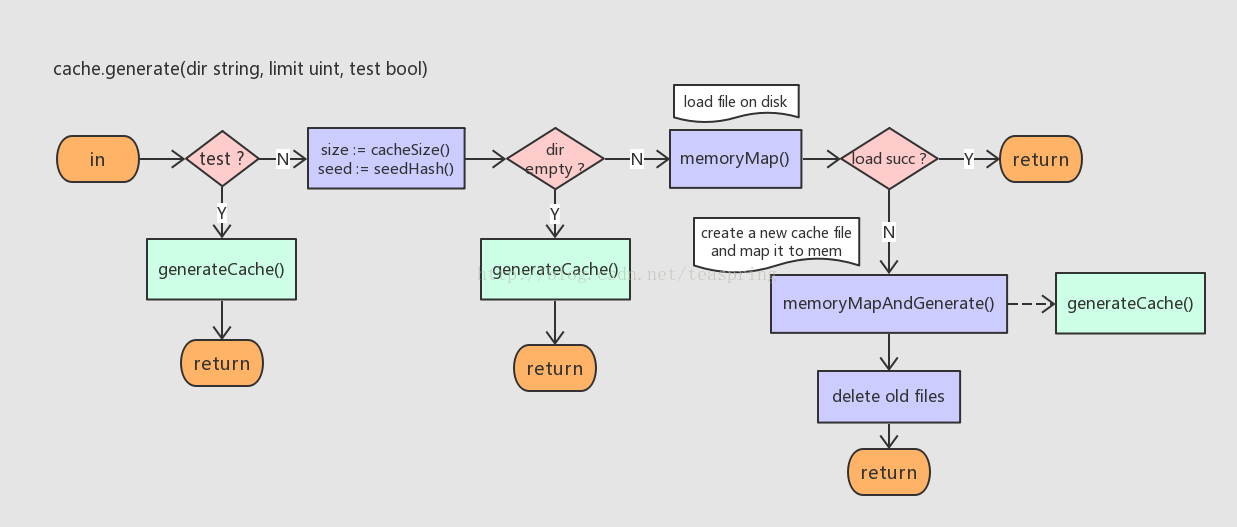
\includegraphics[scale=0.3]{cache_generate.png}
	\caption{cache generate}
	\label{cacheGenerate}
\end{figure}

上图是cache.generate()方法的基本流程:如果是测试用途,则不必考虑磁盘文件,直接调用generateCache()创建buffer;如果文件夹为空,那也没法拼接出文件路径,同样直接调用generateCache()创建buffer;然后根据拼接出的文件路径,先尝试读取磁盘上已有文件,如果成功,说明文件已存在并可使用;如果文件不存在,那只好创建一个新文件,定义文件容量,然后利用内存映射将其导入内存。很明显,直接为cache{]创建buffer的generateCache()函数是这里的核心操作,包括memoryMapAndGenerate()方法,都将generateCache()作为一个函数型参数引入操作的。

\Emph{参数size的生成}

参数size是生成buffer的容量,它在上述cache.generate()中生成。

\begin{lstlisting}

size = cacheSize(epoch * epochLength +1)
...
func cacheSize(block uint64) uint64 {
    epoch := int(block / epochLength)
    if epoch < len(cacheSizes) {
        return cacheSizes[epoch]
    }
    size := uint64(cacheInitBytes + cacheGrowthBytes * uint64(epoch) - hashBytes)
    for !(size/hashBytes).ProbablyPrime(1) {
        size -= 2 * hashBytes
    }
    return size
}

\end{lstlisting}

上述就是生成size的代码,cacheSize()的入参虽然是跟区块Number相关,但实际上对于处于同一epoch组的区块来说效果是一样的,每组个数epochLength。Ethash在代码里预先定义了一个数组cacheSizes[],存放了前2048个epoch组所用到的cache size。如果当前区块的epoch处于这个范围内,则取用之;若没有,则以下列公式赋初始值。

\begin{center}
$size = cacheInitBytes + cacheGrowthBytes * epoch - hashBytes$
\end{center}

这里$cacheInitBytes = 2^{24}$,$cacheGrowthBytes = 2^{17}$,hashBytes = 64,可见size的取值有多么巨大了。注意到cacheSize()中在对size赋值后还要不断调整,保证最终size是个质数,这是出于密码学的需要。

粗略计算一下size的取值范围,$size = 2^{24} + 2^{17} * epoch$,由于$epoch > 2048 = 2^{11}$,所以$size  > 2^{28}$,生成的buffer至少有256MB,而这还仅仅是VerifySeal()使用的cache{},Seal()使用的dataset{}还要大的多,可见这些数据集有多么庞大了。

\Emph{参数seed[]的生成}

参数seed是generateCache()中对buffer进行哈希运算的种子数据,它也在cache.generate()函数中生成。

\begin{lstlisting}

seed := seedHash(epoch * epochLength +1)
...
func seedHash(block uint64) []byte {
    seed := make([]byte, 32)
    if block < epochLength { // epochLength = 30000
        return seed
    }
    keccak256 := makeHasher(sha3.NewKeccak256())
    for i := 0; i < int(block/epochLength); i++ {
        keccak256(seed, seed)
    }
    return seed
}
type hasher func(dest []byte, data []byte)
func makeHasher(h hash.Hash) hasher {
    return func(dest []byte, data []byte) {
        h.Write(data)
        h.Sum(dest[:0])
        h.Reset()
    }
}


\end{lstlisting}

上述seedHash()函数用来生成所需的seed[]数组,它的长度32bytes,与common.Address类型长度相同。makeHasher()函数利用入参的哈希函数接口生成一个哈希函数,这里用了SHA3-256哈希函数。注意seedHash()中利用生成的哈希函数keccak256()对seed[]做的原地哈希,而原地哈希运算的次数跟当前区块所处的epoch序号有关,所以每个不同的cache{}所用到的seed[]也是完全不同的,这个不同通过更多次的哈希运算来实现。


\Emph{generateCache()函数}


generateCache()函数在给定种子数组seed[]的情况下,对固定容量的一块buffer进行一系列操作,使得buffer的数值分布变得随机、无规律可循,最终buffer作为cache{}中的数组(非线性表)返回,还可作为数据源帮助生成dataset{}。generateCache()函数主体分两部分,首先用SHA3-512哈希函数作为哈希生成器(hasher),对buffer数组分段(每次64bytes)进行哈希化,然后利用StrictMemoryHardFunction中的RandMemoHash算法对buffer再进行处理。这个RandMemoHash算法来自2014年密码学方向的一篇学术论文,有兴趣的朋友可以搜搜看。

\Emph{内存映射}

由于Ethash(PoW)算法中用到的随机数据集cache{}和dataset{}过于庞大,将其以文件形式存储在磁盘上就显得很有必要。同样由于这些文件过于庞大,使用时又需要一次性整体读入内存(因为对其的使用是随意截取其中的一段数据),使用内存映射可以大大减轻I/O负担。cache{}和dataset{}结构体中,均有一个mmap对象用以操作内存映射,以及一个系统文件对象dump,对应于打开的磁盘文件。



\Emph{Ethash算法总结:}

回看一下Ethash共识算法最基本的形态,如果把整个result[]的生成过程视作那个概念上的函数RAND(),则如何能更加随机,分布更加均匀的生成数组,关系到整个Ethash算法的安全性。毕竟如果result[]生成过程存在被破译的途径,那么必然有方法可以更快地找到符合条件的数组,通过更快的挖掘出区块,在整个以太坊系统中逐渐占据主导。所以Ethash共识算法应用了非常复杂的一系列运算,包含了多次、多种不同的哈希函数运算:

\begin{itemize}

\item 大量使用SHA3哈希函数,包括256-bit和512-bit形式的,用它们来对数据(组)作哈希运算,或者充当其他更复杂哈希计算的某个原型 -- 比如调用makeHasher()。而SHA3哈希函数,是一种典型的可应对长度变化的输入数据的哈希函数,输出结果长度统一(可指定256bits或512bits)。

\item lookup()函数提供了非线性表格查找方式的哈希函数,相关联的dataset{}和cache{}规模巨大,其中数据的生成/填充过程中也大量使用哈希函数。

\item 在一些计算过程中,有意将[]byte数组转化为uint32或uint64整型数进行操作(比如XOR,以及类XOR的FNV()函数)。因为理论证实,在32位或64位CPU机器上,以32位/64位整型数进行操作时,速度更快。
\end{itemize}

\paragraph{Clique共识算法}
Clique算法又称Proof-of-Authortiy(PoA),它实现的Seal()其实是一个标准的数字签名加密过程,可由下列公式表示:

\begin{center}
$n = F(pr, h)$
\end{center}

其中F()是数字签名函数,n是生成的数字签名,pr是公钥,h是被加密的内容。具体到Clique应用中,n是一个65 bytes长的字符串,pr是一个common.Address类型的(长度20 bytes)地址,h是一个common.Hash类型(32 bytes)的哈希值,而签名算法F(),目前采用的正是\Emph{椭圆曲线数字签名算法}(ECDSA)。

没错,就是这个被用来生成交易(Transaction)对象的数字签名的ECDSA。在Clique的实现中,这里用作公钥的Address类型地址有一个限制,它必须是已认证的(authorized)。所以Clique.Seal()函数的基本逻辑就是:有一个Address类型地址打算用作数字签名的公钥(不是区块的作者地址Coinbase);如果它是已认证的,则执行指定的数字签名算法。而其中涉及到的动态管理所有认证地址的机制,才是Clique算法(PoA)的精髓。

\Emph{基于投票的地址认证机制}

首先了解一下Clique的认证机制authorization所包括的一些设定:

\begin{itemize}

\item 所有的地址(Address类型)分为两类,分别是经过认证的,和未经过认证的。

\item 已认证地址(authorized)可以变成未认证的,反之亦然。不过这些变化都必须通过投票机制完成。

\item 一张投票包括:投票方地址,被投票地址,和被投票地址的新认证状态。有效投票必须满足:被投票地址的新认证地址与其现状相反。

\item 任意地值A只能给地址B投一张票
\end{itemize}

这些设定理解起来并不困难,把这里的地址替换成平常生活中的普通个体,这就是个很普通的投票制度。Clique算法中的投票系统的巧妙之处在于,每张投票并不是某个投票方主动“投”出来的,而是随机组合出来的。

想了解更多细节免不了要深入一些代码,下图是Clique算法中用到的一些结构体:

\begin{figure}
	\centering
	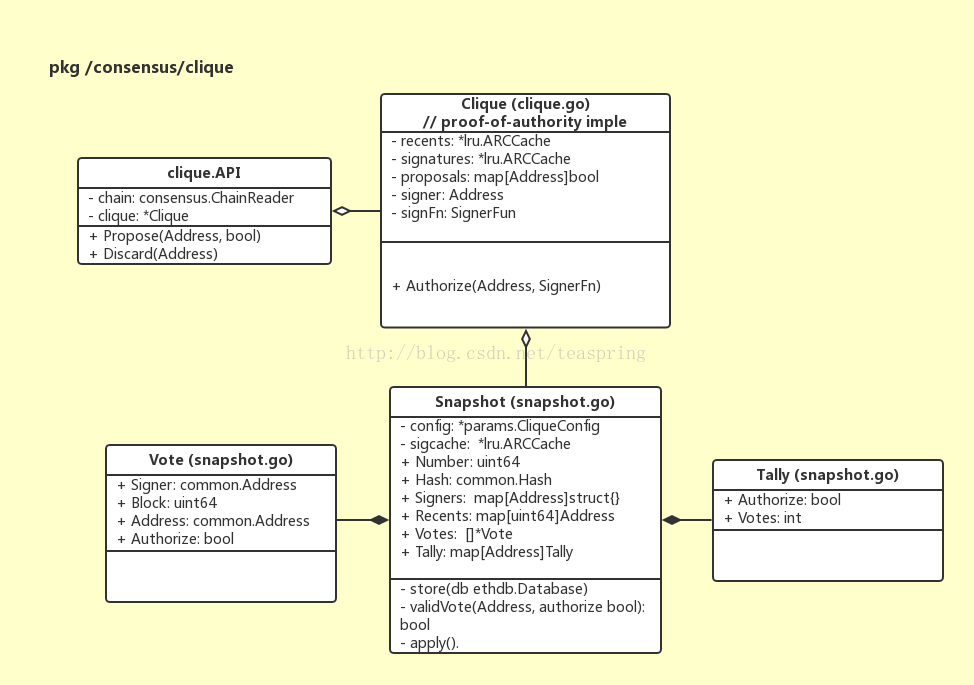
\includegraphics[scale=0.4]{clique.png}
	\caption{clique}
	\label{clique}
\end{figure}

Clique结构体实现了共识算法接口Engine的所有方法,它可对区块作Seal操作。它的成员signFn正是数字签名生成函数,signer用作数字签名的公钥,这两成员均由Authorize()函数进行赋值。它还有一个map类型成员proposals,用来存放所有的不记名投票,即每张投票只带有被投票地址和投票内容(新认证状态),由于是map类型,显然这里的proposals存放的是内容不同的不记名投票。API结构体对外提供方法,可以向Clique的成员变量proposals插入或删除投票。

Snapshot结构体用来动态管理认证地址列表,在这里认证地址是分批次存储和更新的,一个Snapshot对象,存放的是以区块为时序的所有认证地址的"快照"。Snapshot的成员Number和Hash,正是区块Block的标志属性;成员Signers存储所有已认证地址。

一个Vote对象表示一张记名投票。Tally结构体用来记录投票数据,即某个(被投票)地址总共被投了多少票,新认证状态是什么。Snapshot中用map型变量Tally来管理所有Tally对象数据,map的key是被投票地址,所以Snapshot.Tally记录了被投票地址的投票次数。另外Snapshot还有一个Vote对象数组,记录所有投票数据。

\Emph{新区块的Coinbase是一个随机的被投票地址}

Engine接口的Prepare()方法,约定在Header创建后调用,用以对Header的一些成员变量赋值,比如作者地址Coinbase。在Clique算法中,新区块的Coinbase来自于proposals中的某个被投票地址。

\begin{figure}
	\centering
	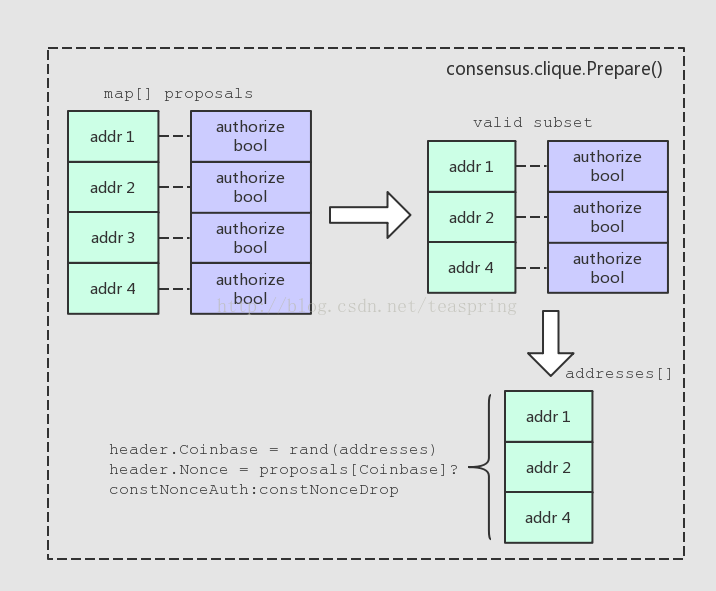
\includegraphics[scale=0.5]{clique_coinbase.png}
	\caption{clique coinbase}
	\label{cliqueCoinbase}
\end{figure}

上图解释了Clique.Prepare()方法中的部分逻辑。首先从proposals中筛选出有效的不记名投票,要么是已认证地址变为未认证,要么反过来;然后获取有效的被投票地址列表,从中随机选取一个地址作为该区块的Coinbase,与之相应的投票内容则被区块的Nonce属性携带。而新区块的Coinbase会在之后的更新认证地址环节,被当作一次投票的被投票地址。

ps,Ethash算法中,新区块的Coinbase地址可是异常重要的,因为它会作为新区块的作者地址,被系统奖励或补偿以太币。但Clique算法中就完全不同了,由于工作在测试网络中,每个帐号地址获得多少以太币没有实际意义,所以这里的Coinbase任意赋值倒也无妨。

\Emph{添加记名投票并更新认证地址列表}

管理所有认证地址的结构体是Snapshot,具体到更新认证地址列表的方法是apply()。它的基本流程如下图:

\begin{figure}
	\centering
	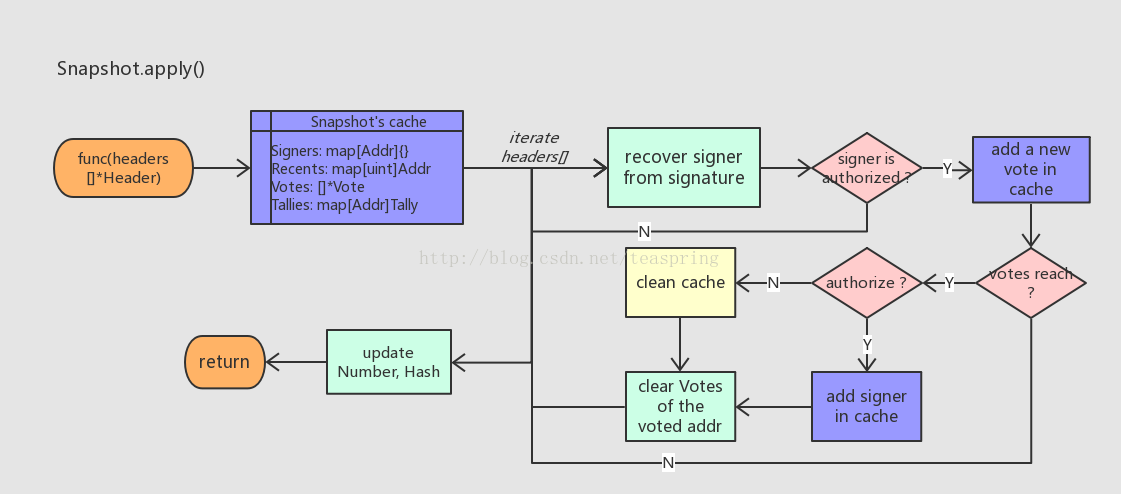
\includegraphics[scale=0.3]{snapshot.png}
	\caption{Snapshot}
	\label{snapshot}
\end{figure}

重温一下Snapshot结构体内声明的一组缓存成员变量:

\Emph{Signers}是全部已认证地址集合,注意这里用map类型来提供Set的行为。

\Emph{Recents}用来记录最近担当过数字签名算法的signer的地址,通过它Snapshot可以控制某个地址不会频繁的担当signer。更重要的是,由于signer地址会充当记名投票的投票方,所以Recents可以避免某些地址频繁的充当投票方!Recents中map类型的key是区块Number值。

\Emph{Votes}记录了所有尚未失效的记名投票;Tallies记录了所有被投票地址(voted)目前的(被)投票次数。

Snapshot.apply()函数的入参是一组Header对象,它们来自区块主链上按从旧到新顺序排列的一组区块,并且严格衔接在Snapshot当前状态(成员Number,Hash)之后。注意,这些区块都是当前“待挖掘”新区块的祖先,所以它们的成员属性都是已经确定的。apply()方法的主要部分是迭代处理每个Header对象,处理单个Header的流程如下:

\begin{itemize}

\item 首先从数字签名中恢复出签名所用公钥,转化为common.Address类型,作为signer地址。数字签名(signagure)长度65 bytes,存放在Header.Extra[]的末尾。

\item 如果signer地址是尚未认证的,则直接退出本次迭代;如果是已认证的,则记名投票+1。所以一个父区块可添加一张记名投票,signer作为投票方地址,Header.Coinbase作为被投票地址,投票内容authorized可由Header.Nonce取值确定。

\item 更新投票统计信息。如果被投票地址的总投票次数达到已认证地址个数的一半,则通过之。

\item 该被投票地址的认证状态立即被更改,根据是何种更改,相应的更新缓存数据,并删除过时的投票信息。

\end{itemize}

在所有Header对象都被处理完后,Snapshot内部的Number,Hash值会被更新,表明当前Snapshot快照结构已经更新到哪个区块了。

Snapshot.apply()方法在Clique.Seal()中被调用,具体位于运行数字签名算法之前,以保证即将充当公钥的地址可以用最新的认证地址列表加以验证。



综上所述,Clique算法在投票制度的安全性设计上完善了诸多细节:

\begin{itemize}

\item 外部参与不记名投票的方式是通过API.Propose(),Discard()来操作Clique.proposals。由于proposals是map类型,所以每个投票地址(map的key)在proposals中只能存在一份,这样就杜绝了外部通过恶意操作Clique.proposals来影响不记名投票数据的企图。

\item 所有认证地址的动态更新,由一张张记名投票累计作用影响。而每张记名投票的投票方地址和投票内容(不记名投票),是以毫不相关、近乎随机的方式组合起来的。所以,理论上几乎不存在外部恶意调用代码从而操纵记名投票数据的可能。同时,通过一些内部缓存(Snapshot.Recents),避免了某些signer地址过于频繁的充当投票方地址。

\end{itemize}

虽然Clique共识算法并非作用在产品环境,但它依然很精巧的设计了完整的基于投票的选拔制度,很好的践行了"去中心化"宗旨。这对于其他类型共识算法的设计,提供了一个不错的样本。

\Emph{小结}

本篇介绍了挖掘一个新区块在代码上的完整过程,从调用函数入口开始,沿调用过程一路向深,直至最终完成新区块授权/封印的共识算法,并对两种共识算法的设计思路和实现细节都进行了详细讲解。

\begin{itemize}

\item 一般所说的“挖掘一个新区块”其实包括两部分,第一阶段组装出新区块的所有数据成员,包括交易列表txs、叔区块uncles等,并且所有交易都已经执行完毕,各帐号状态更新完毕;第二阶段对该区块进行授勋/封印(Seal),没有成功Seal的区块不能被广播给其他节点。第二阶段所消耗的运算资源,远超第一阶段。

\item Seal过程由共识算法(consensus algorithm)族完成,包括Ethash算法和Clique算法两种实现。前者是产品环境下真实采用的,后者是针对测试网络(testnet)使用的。Seal()函数并不会增加或修改区块中任何跟有效数据有关的部分,它的目的是通过一系列复杂的步骤,或计算或公认,选拔出能够出产新区块的个体。

\item \Emph{Ethash算法(PoW)基于运算能力来筛选出挖掘区块的获胜者},运算过程中使用了大量、多次、多种的哈希函数,通过极高的计算资源消耗,来限制某些节点通过超常规的计算能力轻易形成“中心化”倾向。

\item \Emph{Clique算法(PoA)利用数字签名算法完成Seal操作},不过签名所用公钥,同时也是common.Address类型的地址必须是已认证的。所有认证地址基于特殊的投票地址进行动态管理,记名投票由不记名投票和投票方地址随机组合而成,杜绝重复的不记名投票,严格限制外部代码恶意操纵投票数据

\item 在实践“去中心化”方面,以太坊还在区块结构中增加了叔区块(uncles)成员以加大计算资源的消耗,并通过在交易执行环节对叔区块作者(挖掘者)的奖励,以收益机制来调动网络中各节点运算资源分布更加均匀。

\end{itemize}

\ifx\allfiles\undefined
\end{document}
\fi